%% LaTeX-Beamer template for KIT design
%% by Erik Burger, Christian Hammer
%% title picture by Klaus Krogmann
%%
%% version 2.1
%%
%% mostly compatible to KIT corporate design v2.0
%% http://intranet.kit.edu/gestaltungsrichtlinien.php
%%
%% Problems, bugs and comments to
%% burger@kit.edu

\documentclass[18pt]{beamer}

\usepackage{tikz}

%% SLIDE FORMAT

% use 'beamerthemekit' for standard 4:3 ratio
% for widescreen slides (16:9), use 'beamerthemekitwide'

\usepackage{templates/beamerthemekit}
% \usepackage{templates/beamerthemekitwide}

% DEUTSCHE SPRACHE EINBINDEN
\usepackage[utf8]{inputenc}

% Deutsche Ausgabe anpassen
\usepackage[T1]{fontenc}

%% TITLE PICTURE

% if a custom picture is to be used on the title page, copy it into the 'logos'
% directory, in the line below, replace 'mypicture' with the 
% filename (without extension) and uncomment the following line
% (picture proportions: 63 : 20 for standard, 169 : 40 for wide
% *.eps format if you use latex+dvips+ps2pdf, 
% *.jpg/*.png/*.pdf if you use pdflatex)

%\titleimage{mypicture}

%% TITLE LOGO

% for a custom logo on the front page, copy your file into the 'logos'
% directory, insert the filename in the line below and uncomment it

\titlelogo{mj++logo}

% (*.eps format if you use latex+dvips+ps2pdf,
% *.jpg/*.png/*.pdf if you use pdflatex)

%% TikZ INTEGRATION

% use these packages for PCM symbols and UML classes
% \usepackage{templates/tikzkit}
% \usepackage{templates/tikzuml}

% the presentation starts here

\title[]{mj++}
\subtitle{Compilerpraktikum WS 2014/15}
\author{Gruppe 5: mj++}
\date{10. Februar 2015}

\institute{Institut für Programmstrukturen und Datenorganistation}

% Bibliography

%\usepackage[citestyle=authoryear,bibstyle=numeric,hyperref,backend=biber]{biblatex}
%\addbibresource{templates/example.bib}
%\bibhang1em

\usepackage{courier}
\usepackage{listings}
\lstset{frame=single,basicstyle=\small\ttfamily,language=Java}

\usepackage{xcolor}
\definecolor{lightgray}{gray}{0.9}
\definecolor{kitblue}{RGB}{227, 232, 242}
\newcommand{\code}[1]{\colorbox{lightgray}{\texttt{\upshape #1}}}
\newcommand{\token}[1]{\colorbox{kitblue}{\texttt{\upshape #1}}}

\begin{document}

\selectlanguage{ngerman}

\begin{frame}
\titlepage
\end{frame}

\begin{frame}{Outline}
\tableofcontents
\end{frame}

\section{MiniJava}

\begin{frame}
    \frametitle{MiniJava}
    \begin{itemize}
        \item MiniJava $\subsetneq$ Java
        \item Typen: \code{int}, \code{boolean}, Arrays, Objekte
            \begin{itemize}
                \item \emph{nicht}: \code{String}, \code{double}, \code{float}, \ldots
            \end{itemize}
        \item keine Vererbung, Interfaces, Exceptions, \ldots
        \item nur \code{public}-Member
        \item keine \code{static}-Methoden
        \item nicht alle Operatoren (z.B.\ \code{++})
    \end{itemize}
    \vskip 1cm
    \begin{center}
        Ziel: MiniJava auf x86\_64 kompilieren
    \end{center}
\end{frame}

\section{Lexikalische Analyse}
\begin{frame}
    \frametitle{Lexikalische Analyse}
    \framesubtitle{Überblick}
    \lstinputlisting{foo.mj}
    \pause
     \begin{tabular}{lllllll}
         \visible<2->{\token{class}} & \visible<3->{\token{Foo}} & \visible<4->{\token{\{}} & \visible<5->{\token{public}} & \visible<6->{\token{int}} & \visible<7->{\token{bar}} & \visible<8->{\token{(}}\\
         \only<2>{\texttt{KEYWORD\_CLASS}} & \only<3>{\texttt{IDENT}} & \only<4>{\texttt{L\_BRACE}} & \only<5>{\texttt{KEYWORD\_PUBLIC}} & \only<6>{\texttt{KEYWORD\_INT}} & \only<7>{\texttt{IDENT}} & \only<8>{\texttt{L\_PAREN}}
     \end{tabular}
\end{frame}

\begin{frame}[t]
    \frametitle{Lexikalische Analyse}
    \framesubtitle{Ansätze}
    \vskip .4cm
    Endlicher Automat
    \begin{itemize}
        \item<2-> Ausprogrammieren
            \only<2>{
                \lstinputlisting[basicstyle=\ttfamily\scriptsize,language=C]{lexer-switch-case.code}
            }
        \item<3-> Tabelle
            \only<4->{
            \begin{tikzpicture}[overlay]
                \node at (.8,.2) {
\includegraphics[angle=15,origin=c,width=1.5cm,keepaspectratio=true]{logos/mj++logo.png}};
            \end{tikzpicture}
        }
            \lstinputlisting[basicstyle=\ttfamily\scriptsize,language=C]{lexer-table.code}
        \item<5-> woher kommt die Tabelle?
            \begin{itemize}
                \item<6-> Graph zusammenklicken $\Rightarrow$ daraus Tabelle bauen
            \end{itemize}
    \end{itemize}
\end{frame}

\begin{frame}
    \frametitle{Lexikalische Analyse}
    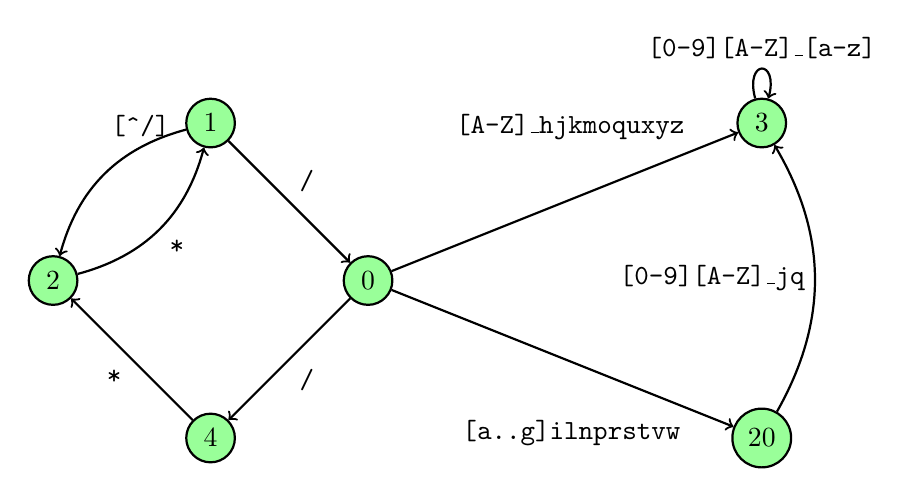
\begin{tikzpicture}
        \node[circle,thick,draw=black,fill=green!40] (0) at (0,0) {0};
        \node[circle,thick,draw=black,fill=green!40] (1) at (-2,2) {1};
        \node[circle,thick,draw=black,fill=green!40] (2) at (-4,0) {2};
        \node[circle,thick,draw=black,fill=green!40] (4) at (-2,-2) {4};
        \node[circle,thick,draw=black,fill=green!40] (3) at (5,2) {3};
        \node[circle,thick,draw=black,fill=green!40] (20) at (5,-2) {20};
        \draw[thick,->] (0) to              node[midway,anchor=north west] {\texttt{/}} (4);
        \draw[thick,->] (4) to              node[midway,anchor=north east] {\texttt{*}} (2);
        \draw[thick,->] (2) to [bend right] node[midway,anchor=north west] {\texttt{*}} (1);
        \draw[thick,->] (1) to [bend right] node[near start,anchor=south] {\texttt{[\^{}/]}}           (2);
        \draw[thick,->] (1) to              node[midway,anchor=south west] {\texttt{/}} (0);
        \draw[thick,->] (0) to              node[very near end,anchor=north east] {\texttt{[a..g]ilnprstvw}} (20);
        \draw[thick,->] (0) to node[very near end,anchor=south east] {\texttt{[A-Z]\_hjkmoquxyz}} (3);
        \draw[thick,->] (20) to [bend right] node[midway,anchor=east] {\texttt{[0-9][A-Z]\_jq}} (3);
        \draw[thick,->] (3) to [loop above] node {\texttt{[0-9][A-Z]\_[a-z]}} (3);
    \end{tikzpicture}
\end{frame}

\begin{frame}[t]
    \frametitle{Lexikalische Analyse}
    \vskip 1.8cm
    Zwei Ansätze:
    \begin{itemize}
        \item<1-> Push-Interface
            \only<1>{
                \\[3pt] \code{void handle\_token(token t);}
                \\[3pt] \code{void lex(F callback);}
            }
        \item<2-> Pull-Ansatz
            \only<3>{
                \begin{tikzpicture}[overlay]
                    \node at (.8,.2) {
\includegraphics[angle=10,origin=c,width=1.5cm,keepaspectratio=true]{logos/mj++logo.png}};
                \end{tikzpicture}
            }
            \only<2->{
                \\[3pt] \code{token get\_next\_token();}
            }
    \end{itemize}
\end{frame}

\begin{frame}
    \frametitle{Lexikalische Analyse}
    \framesubtitle{Erfahrung}
    \begin{itemize}
        \item ohne Keyword-Unterscheidung sehr schnell
        \item Keyword-Unterscheidung aufwändig\\[1pt]
            \hskip .5cm $\Rightarrow$ dedizierte Keyword-Tabelle
        \item für Operatoren kleine Maps
        \item Graph-Dumping zum Debuggen sinnvoll
    \end{itemize}
\end{frame}


\section{Syntaktische Analyse}
\begin{frame}
    \frametitle{Syntaktische Analyse}
    \begin{itemize}
    \item Prüfung, ob Eingabeprogramm syntaktisch korrekt ist
    \item Verschiedene Arten von Parsern
    	\begin{itemize}
    	\item LL(1)- und (S)LL(k)-Parser
    	\item LALR- und LR-Parser
    	\end{itemize}
    \item MiniJava-Grammatik in SLL(3) umformbar \pause
    \item mögliche Technologien
	    \begin{itemize}
		\item Tabellenbasiert
		\item rekursiver Abstieg
    	\end{itemize}
    \item hier handimplementiert mit rekursivem Abstieg
    \end{itemize}
\end{frame}

\begin{frame}
	\frametitle{AST-Aufbau}
	\begin{itemize}
	\item Quelltext muss in passenderes Format umgewandelt werden
	\item Zeichen und Regeln ohne Bedeutung werden nicht übernommen
	\item Ergebnis ist der abstrakte Syntaxbaum (AST)
	\item Aufbau während des Parsens
	\end{itemize}
\end{frame}

\begin{frame}
	\frametitle{Beispiel}
	\token{class}, \token{Foo}, \token{\{}, \token{public}, \token{int}, \token{bar}, \token{(}, \token{)}, \token{\{}, \ldots \\
            \texttt{KEYWORD\_CLASS}, \texttt{IDENT}, \texttt{L\_BRACE}, \ldots \\
     wird zu \\
     \begin{center}
     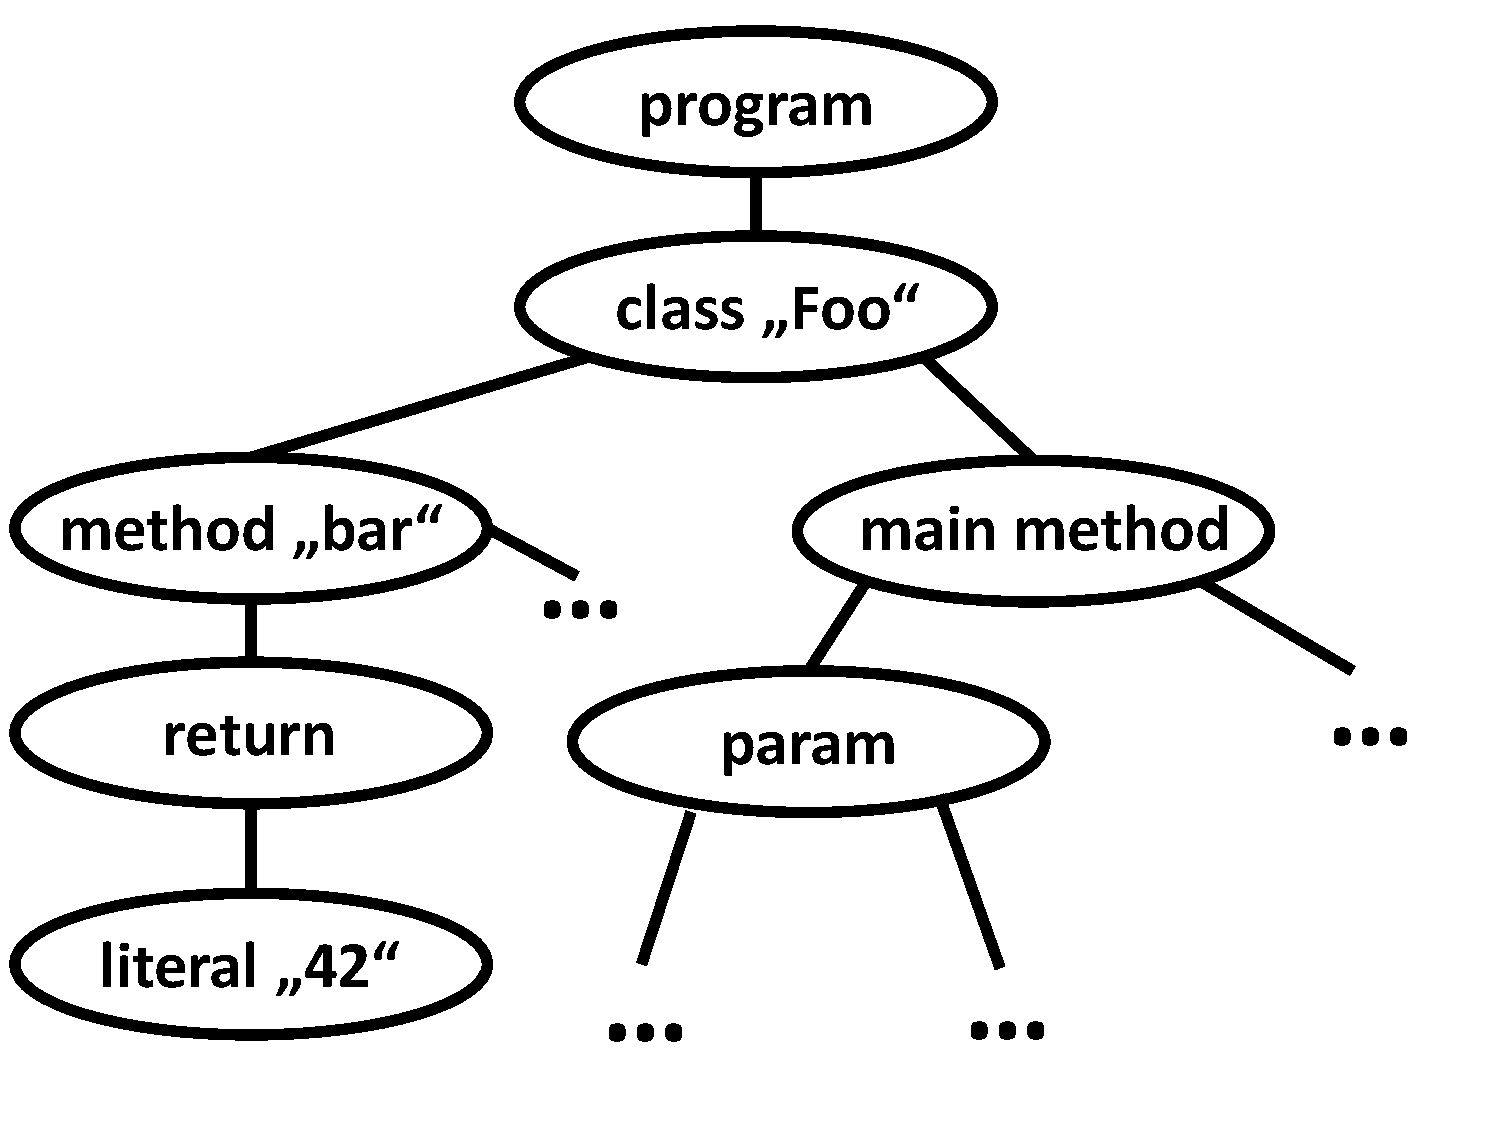
\includegraphics[scale=0.3]{images/AST.pdf}
     \end{center}
\end{frame}

\section{Besonderheiten von mj++}
\begin{frame}
	\frametitle{Zahlen, Daten, Fakten} % Dummer Titel, mir fällt aber nichts besseres ein.
	\begin{itemize}
		\item Laufzeitanteil von Lexer und Parser: $\approx$ 5-10\%	%falls wir das separat messen: in je 1 Zeile schreiben
		\item LoC (gesamt): ca. 12,5k-13k (letzte Zählung: 12836)
		\item verwendete Tools: 
		\begin{itemize}
			\item Git
			\item Issue-Tracker
			\item astyle
			\item gprof
			\item \dots
		\end{itemize}
	\end{itemize}
\end{frame}

\begin{frame}
    \frametitle{Besonderheiten von mj++}
    \begin{itemize}
        \item (einfache) Error-Recovery im Parser zur Meldung verschiedener Fehler
        \begin{itemize}
        	\item Beispiel: \code{public static 42 void main...}
        \end{itemize} \pause
        \item Semantische Analyse von Expression-Statements und Definite-Return-Analysis nahe an Java-Semantik
        \begin{itemize}
        	\item Verbot von Expressions wie \code{4+2;} oder \code{a;} (siehe JLS §15.2ff)
        	\item Definite-Return-Analysis: \lstinputlisting{DRA.mj}
        \end{itemize} \pause
        \item schnelle Compilation
            \pause
        \begin{itemize}
        \item Gruppe 5 sind die Besten!
            \begin{tikzpicture}[overlay]
                \node at (.8,.2) {
\includegraphics[angle=-10,origin=c,width=1.5cm,keepaspectratio=true]{logos/mj++logo.png}};
            \end{tikzpicture}
        \end{itemize}
    \end{itemize}
\end{frame}

\end{document}
